\documentclass[a4paper,14pt]{extarticle}
\usepackage[margin=1in]{geometry}
\usepackage{amsmath}
\usepackage{enumitem}
\usepackage{tcolorbox}
\usepackage{fancyhdr}
\usepackage{titlesec}
\usepackage{hyperref}
\hypersetup{colorlinks=true, urlcolor=blue, linkcolor=black}

\usepackage{amsmath, amssymb}  % Enables \mathbb, \rightarrow, etc.

\usepackage{listings}

\usepackage{float}

\usepackage{listings}
\usepackage{xcolor}  % For color customization

%--------------- using "-" as labes in \begin{enumerate}[label=-]
\usepackage{enumitem}  % In preamble

\usepackage{graphicx}
\usepackage{caption}

\lstset{
  language=C,
  basicstyle=\ttfamily\small,
  keywordstyle=\color{black},
  stringstyle=\color{black},
  commentstyle=\color{black}\itshape,
  numbers=left,
  numberstyle=\tiny,
  stepnumber=1,
  numbersep=5pt,
  showstringspaces=false,
  breaklines=true,
  frame=single,
  tabsize=2
}

\usepackage{fancyhdr}
\setlength{\headheight}{17pt}  % Fix warning from fancyhdr
\pagestyle{fancy}
\fancyhf{}
\rhead{The Art of Electronics}
% \lhead{Short Notes}
\rfoot{Page \thepage}
\lfoot{@varunjha089}


\title{The Art of Electronics}
\author{Paul Horowitz and Winfield Hill}
\date{Start Date: July 16, 2025 $\|$ Last Modified: \today}



\begin{document}

\maketitle
\tableofcontents
% \newpage
\listoffigures
\newpage


\newpage
\lhead{Digital Logic}
\section{Digital Locic}
\subsection{Basic Logic Concept}
\subsubsection{Digital versus Analog}

Thus far we have been dealing with circuit in which the input and output voltages have varied over a continuous range of values:

\begin{enumerate}[label=(\alph*)]
    \item RC Circuti
    \item amplifiers
    \item integrators
    \item rectifiers
    \item op-amp
\end{enumerate}

\noindent This is natural when dealing with signals that are continuous (e.g., audio\\
 signal) or continuously varying voltages from measuring instrument\\ 
 (e.g., temperataure-reading or light-detecting devices, or biological or\\ chemical probe).

However, there are instances in which the input signal is naturally discrete in form 
e.g., Pulse from a Particle Detector, or "bits" of data from a switch, keybord, or 
computer. Furthermore, it is often desirable to convert continuous (analog) data to digital form, and vice versa using 
Digital-to-Analog Convertres (DACs) or Analog-to-Digital Convertres (ADCs).

Another interesting example of the power of digital techniques is the transmission of analog signals without 
degradation by noise: an analog audio or video signal, for instance, picks up "noise" while being transmitted
by cable or wireless that cannot be removed. If, instead, the signal is converted to a series of numbers
representing its amplitude at successive instants of time, and these numbers are transmitted as digital
signal, the analog signal reconstruction at the receiving end (done with DACs) will be without error, providing
the noise level on the transmission channel isn't great enough to prevent accurate recognition of 1s and 0s.
This technique, known as PCM (Pulse-Code-Modulation), is particularly attractive where a signal must pass 
through a series of "repeaters", simce digital regeneration at each stage gurantees noiseless transmission.

The information and stunning pictures sent back by planetary deep space probes, for example the Pioneer 10
mission to Jupiter in 1973, were stored and transmitted with PCM.

\newpage
\lhead{10.1 Basic Logic Concept}
\subsubsection{Logic States}
By "Digital Electronics" we means circuit in which there are only two (usually) states possible at any 
point e.g., a transistor that can either be in saturation or be nonconducting.

\subsubsection*{A. HIGH and LOW}
The HIGH and LOW voltage states represent the TRUE and FALSE states of Boolean logic, in some predefined way.
If at some point a HIGH voltage represents TRUE, that signal line is called "actice high" (or "HIGH true") 
Figure below shows an example. SWITCH CLOSED is true when the output is low; that's an "active-LOW" 
(or "LOW-true") signal, and you might label the lead as shown (a bar over a symbol means NOT; that line is
HIGH when the swithc is $not$ closed)   

Just remember the presence of \textbf{negation bar} over the label tells whether the wire is at a LOW or HIGH
voltage state when the stated condition (SWITHC CLOSED) is true.\footnote{"Positive-true" and "Negative-ture" used for HIGH-true
and LOW-true, respectively.}

\begin{figure}[h!]
    \centering
    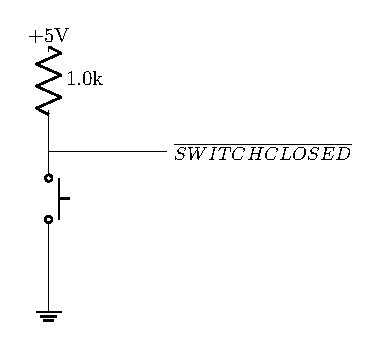
\includegraphics[width=0.5\textwidth]{10.1.pdf}
    \caption{A LOW-true (“active-LOW”) logic level.}
    \label{fig:lowtrue}
\end{figure}

\subsubsection*{B. Voltage range of HIGH and LOW}

\newpage
\lhead{Computer, Controller, and Data Link}
\section{Computer, Controller, and Data Link}

In Ch 14 and 15 we will deal with computer and controllers (with the\\ 
common alternative name of microcontroller).\\

\newpage
\lhead{Microcontrollers}
\section{Microcontrollers}

\end{document}